\documentclass[12pt]{article}
\usepackage{amsmath,amssymb,amsfonts}
\usepackage{graphicx}
\usepackage{geometry}
\geometry{a4paper, margin=1in}
\usepackage{mathrsfs}
\usepackage{tikz}
\usetikzlibrary{arrows.meta, calc, decorations.markings}

% Стиль для стрелок
\tikzset{
    vector/.style={-{Stealth[length=3mm]}, thick, black},
    axis/.style={-{Stealth[length=2.5mm]}, thin, black},
}

\begin{document}

\noindent J. Mech. Phys. Solids Vol. 38, No. 4, pp. 481--490, 1990. \hfill 0022--5096/90 \$3.00 + 0.00 \\
Printed in Great Britain. \hfill \copyright\ 1990 Pergamon Press plc

\vspace{1cm}

\begin{center}
{\Large\bf THE SINGULAR NATURE OF THE STRESS FIELD NEAR AN ARBITRARILY MOVING DISLOCATION LOOP}

\vspace{0.5cm}

{\large XANTHIPPI MARKENSCOFF and LUQUN NI\textdagger}

\vspace{0.3cm}

Department of Applied Mechanics and Engineering Sciences, University of California, San Diego, La Jolla, CA 92093, U.S.A.

\vspace{0.3cm}

(Received 10 May 1989)
\end{center}

\section*{Abstract}

\textsc{It is} proved that, for the most singular $1/\varepsilon$ terms in the stress field at a point near the current position of a moving loop, the loop may be approximated by its tangent translating with the same instantaneous velocity $\mathbf{v}$ and acceleration $\mathbf{a}$ as the loop has at that point, while, as far as the coefficients of the $\ln\varepsilon$ terms are concerned, the loop is approximated by its tangent at that point translating and rotating as the loop, and by its osculating circle expanding with the same instantaneous velocity as the loop.

\section{Introduction}

\textsc{Static} dislocation loops and the stress field that they create have been extensively studied; however, the stresses due to a moving dislocation loop have not been fully analysed so far. Mura (1963) formulated the problem in terms of a dynamic Green's function for an impulsive force in a 3-D space, and gave the solution as an integral over the loop surface and the loop history in time. He then converted the surface integral into a line integral along the loop curve. Special cases of motion of loops have been treated by Madariaga (1976), G\"unther (1968) and Mura (1969); Markenscoff and Clifton (1982) and Markenscoff and Ni (1984) analysed the wavefront behavior of expanding circular loops.

Although for general motion the solution obtained as an integral over the history of the motion cannot be evaluated in closed form, the asymptotic behavior near and far from the loop may be obtained. In a recent paper Callias et al. (1989) obtained the asymptotic expansion of the stress in a position near an arbitrarily moving loop by using singular asymptotics of integrals.

Here we obtain some geometric features of the singular nature of the stress near the arbitrarily moving loop (planar or non-planar), namely the coefficients of the $1/\varepsilon$ and $\ln\varepsilon$ terms for the stress at a field point that is at a distance of $O(\varepsilon)$ from the current position of the loop. It is proved that for the $1/\varepsilon$ terms the loop may be approximated by its tangent, while the coefficients of $\ln\varepsilon$ comprise terms in which the loop is approximated by its tangent (translating and rotating) and its osculating circle expanding with the same velocity as the loop. As an example we obtain the singular terms near a nonuniformly expanding circular loop.

\section{Near-field Expansion of an Arbitrary Moving Loop}

We consider a loop of arbitrary shape (planar or nonplanar) that moves arbitrarily and wish to obtain the singular terms in the stress at a field point $P$ at a distance $\varepsilon\zeta$ which is of $O(\varepsilon)$ from a point $\Sigma$ on the loop (Fig. 1).

\begin{figure}[ht]
\centering
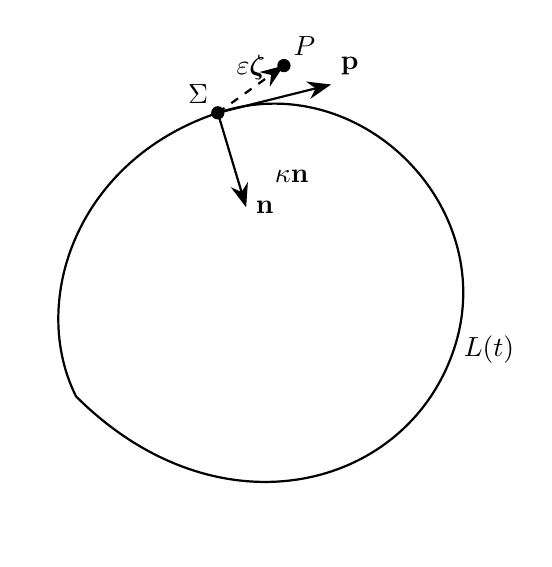
\begin{tikzpicture}[scale=1.2]
    % Произвольная замкнутая петля L(t)
    \draw[thick] 
        (0,0) 
        .. controls (1.5, -1.5) and (3.5, -1) .. (4, 0.5)
        .. controls (4.5, 2) and (3, 3.5) .. (1.5, 3)
        .. controls (0, 2.5) and (-0.5, 1) .. (0, 0);
    
    % Подпись L(t)
    \node[right] at (4, 0.5) {$L(t)$};
    
    % Точка Sigma на петле (верхняя часть)
    \coordinate (Sigma) at (1.5, 3);
    \fill (Sigma) circle (2pt);
    \node[above left] at (Sigma) {$\Sigma$};
    
    % Касательный вектор p
    \draw[vector] (Sigma) -- ++(1.2, 0.3);
    \node[above right] at ($(Sigma)+(1.2, 0.3)$) {$\mathbf{p}$};
    
    % Нормаль n (внутрь петли)
    \draw[vector] (Sigma) -- ++(0.3, -1.0);
    \node[right] at ($(Sigma)+(0.3, -1.0)$) {$\mathbf{n}$};
    
    % Обозначение kappa*n
    \node[below right] at ($(Sigma)+(0.5, -0.5)$) {$\kappa\mathbf{n}$};
    
    % Точка P рядом с Sigma
    \coordinate (P) at (2.2, 3.5);
    \fill (P) circle (2pt);
    \node[above right] at (P) {$P$};
    
    % Вектор от Sigma к P (epsilon*zeta)
    \draw[vector, dashed] (Sigma) -- (P);
    \node[above] at ($(Sigma)!0.5!(P)$) {$\varepsilon\boldsymbol{\zeta}$};
\end{tikzpicture}
\caption{Arbitrary moving loop $L(t)$ with field point $P$ near point $\Sigma$.}
\label{fig:1}
\end{figure}

The near-field asymptotic analysis of this problem is rather lengthy and was performed by Callias et al. (1989); here we analyse the geometric features of the solution by referring to the above reference since the solution discussed here is essentially obtained from it and is too lengthy to reproduce.

The solution of the field quantities strain, stress, velocity are given by Mura (1963) as integrals over the history of the motion:
\begin{equation}
U_{m,n} = \int_{-\infty}^{\infty}\oint_{L(t')} \varepsilon_{njh}C_{ijkl}G_{km,l}(x-x',t-t')b_i\,dl_h\,dt'
+ \int_{-\infty}^{\infty}\oint_{L(t')} \rho G_{im}(x-x',t-t')b_i\varepsilon_{nrs}V_r(x',t')\,dl_s\,dt',
\end{equation}
where $x'$ is a point on the loop at time $t'$, $C_{ijkl}$ the elastic coefficients, $G_{km,l}$ the dynamic Green's function for a point load in a three-dimensional space, $b_i$ the Burgers vector, $\varepsilon_{njh}$ the permutation symbol, $V_r$ the velocity of a point on the loop, $dl_h$ an element of length on the circumference $L(t')$ of the loop.

In order to prove the geometric features of the solution we will use the length of the loop $s$ as a parameter (which is the conventional parameter in differential geometry) instead of the angle $\sigma$ used by Callias et al. (1989), although in many cases using the angle $\sigma$ as a parameter is more intuitive. To obtain the near-field we need to expand the integral in (1) that gives the general solution about the field point $P$. If the length of the loop $s$ is used as a parameter then the integrals in $s$ and $t'$ in (1) are not simply interchangeable since the total length of the loop $L(t')$ at $t'$ is unknown; however we can do the interchange since we only need to evaluate the integral (1) in the neighborhood of the point $\Sigma(s_0,t)$, that is we need to evaluate only
\begin{equation}
\int_{-\infty}^{\infty}\int_{s_0-C}^{s_0+C}(\quad)\,dl_h\,dt',
\end{equation}
where $C>0$ is a suitable constant. Then the interchange of the orders of integration is permissible and we can proceed to perform the integration in $t'$ first, which reduces (2) to an integral in $s$, the asymptotic expansion of which is obtained at $(s_0,t)$. The asymptotic expansions are derived in a similar fashion as in Callias et al. (1989) with some modifications incorporated below and are found to be
\begin{equation}
U_{m,n} = U_{m,n}^{(1)}\cdot\left(\frac{1}{\varepsilon}\right) + (U_{m,n}^{(2)} + U_{m,n}^{(3)})\ln\varepsilon + \text{h.o.t.},
\end{equation}
with
\begin{align*}
U_{m,n}^{(1)} &= \int_0^{\infty}[\hat{F}_2(0,\zeta,c_2) - \hat{F}_2(0,\zeta,c_1) + \hat{F}_5(0,\zeta,c_2) - \hat{F}_5(0,\zeta,c_1) + \hat{F}_4(0,\zeta,c_2)]_{m,n}\,d\zeta, \\
U_{m,n}^{(2)} &= [\hat{F}_1(0,0,c_2) - \hat{F}_1(0,0,c_1) + \hat{F}_3(0,0,c_2)]_{m,n}, \\
U_{m,n}^{(3)} &= \frac{\partial}{\partial\theta}[\hat{F}_2(\theta,0,c_2) - \hat{F}_2(\theta,0,c_1) + \hat{F}_5(\theta,0,c_2) - \hat{F}_5(\theta,0,c_1) + \hat{F}_4(\theta,0,c_2)]_{m,n}\big|_{\theta=0},
\end{align*}
where
\[
\hat{F}_k(\theta,\zeta,c_i) \equiv F_k(\theta,\zeta,c_i) + F_k(-\theta,-\zeta,c_i), \quad k=1,2,3,4,5, \quad i=1,2, \quad \theta = s - s_0
\]
and $F_k(\theta,\zeta,c_i)$ are given in the Appendix. There the following notation are used
\begin{equation}
y = \frac{\varepsilon}{s-s_0} = \frac{\varepsilon}{\theta}, \qquad \Lambda = \frac{t-\tau(s)}{|\varepsilon\zeta + (s-s_0)\mathbf{w}|} = \frac{t-\tau(s)}{|\theta||y\zeta+\mathbf{w}|},
\end{equation}
with $\tau(s)$ satisfying
\begin{equation}
c_i(t-\tau(s)) = |x - x'(s,\tau(s))|, \quad i=1,2,
\end{equation}
\begin{align*}
\mathbf{w} &= y\zeta - \mathbf{p} - \tfrac{1}{2}\mathbf{q}\theta, \\
\mathbf{R} &= \frac{\theta}{|\theta|}\mathbf{w} + (\Lambda\mathbf{v} + \Lambda\mathbf{d}\theta - \tfrac{1}{2}\mathbf{a}\Lambda|\theta||\mathbf{w}|)|\mathbf{w}|, \\
\mathbf{V}^M &= \mathbf{v} + \mathbf{a}\theta - \mathbf{a}\Lambda|\mathbf{w}||\theta|, \\
\mathbf{P} &= \mathbf{p} + \mathbf{q}\theta - \mathbf{a}\Lambda|\mathbf{w}||\theta|,
\end{align*}
\begin{align}
\mathbf{A} &= \mathbf{a} + \frac{\partial^3}{\partial s\,\partial t^2}\mathbf{x}'(s_0,t)\theta - \frac{\partial^3}{\partial t^3}\mathbf{x}'(s_0,t)\Lambda|\mathbf{w}||\theta|, \nonumber \\
\mathbf{D} &= \mathbf{d} + \frac{\partial^3}{\partial s^2\,\partial t}\mathbf{x}'(s_0,t)\theta - \frac{\partial^3}{\partial t^2\,\partial s}\mathbf{x}'(s_0,t)\Lambda|\mathbf{w}||\theta|, \nonumber \\
\Delta &= (c^2-v^2)\Lambda|\mathbf{w}| - 2(\mathbf{d},\mathbf{v})\Lambda|\mathbf{w}|\theta + \tfrac{3}{2}(\mathbf{a},\mathbf{v})\Lambda^2|\mathbf{w}|^2|\theta| \nonumber \\
&\quad - (\mathbf{w},\mathbf{v})\operatorname{sgn}\theta - (\mathbf{w},\mathbf{d})|\theta| + (\mathbf{a},\mathbf{w})\Lambda|\mathbf{w}|\theta
\end{align}
and
\begin{equation}
\begin{aligned}
\frac{\partial}{\partial t}\mathbf{x}(s_0,t) &\equiv \mathbf{v}, \\
\frac{\partial^2}{\partial t^2}\mathbf{x}(s_0,t) &= \mathbf{a}, \\
\frac{\partial}{\partial s}\mathbf{x}(s_0,t)\big|_{s=s_0} &\equiv \mathbf{p} \quad \text{with } |\mathbf{p}|=1, \\
\frac{\partial^2}{\partial s^2}\mathbf{x}(s,t)\big|_{s=s_0} &\equiv \mathbf{q} = \kappa\mathbf{n}, \\
\frac{\partial^2}{\partial s\,\partial t}\mathbf{x}(s,t)\big|_{s=s_0} &= \frac{\partial\mathbf{p}}{\partial t} \equiv \mathbf{d}.
\end{aligned}
\end{equation}

We observe that $\mathbf{p}$ is the unit tangent to the loop at $s_0$, $\kappa=\kappa(s_0)$ is the curvature of the loop at $s_0$, and $\mathbf{n}$ is the unit normal to the loop at that point. For these quantities to be uniquely defined, at that point the loop must have up to the third-order continuous derivatives with respect to $s$ and $t$.

Now, we are going to prove our conclusion about the geometric features of the singular terms in (3). From (3), it may be readily seen that the coefficients of $1/\varepsilon$ are integrals of $F_2, F_4, F_5$, therefore of $F_2, F_4, F_5$, evaluated at $\theta=0$ (i.e. $s=s_0$). We consider the integral of $F_2$ first. From (A2) in the Appendix, we observe that $F_2$ depends on $\mathbf{V}^M$, $\mathbf{P}$, $\mathbf{W}$, $\mathbf{R}$, $\Delta$ and $\Lambda$ in the limit as $\theta\to 0$. Considering that
\[
\Lambda_1 = \lim_{\theta\to 0}\Lambda = \frac{1}{c_i^2-v^2}\left\{\frac{(s\mathbf{w},\mathbf{v})}{s\mathbf{w}} + \sqrt{\left(\mathbf{v},\frac{\mathbf{w}}{|\mathbf{w}|}\right)^2 + c_i^2 - v^2}\right\}
\]
(see Callias et al., 1989, for Eq. (37)), and (6) in the limit as $\theta\to 0$, it can be seen that $F_2$ and its integral are only dependent on $\mathbf{p}$, $\mathbf{v}$, $\zeta$ and $c_t$. Similar discussions apply to the integrals of $F_4$ and $F_5$. Therefore, we can state that the most singular $1/\varepsilon$ terms for the arbitrary moving loop near a point $\Sigma$ are the same as those of the tangent dislocation at $\Sigma$ moving steadily with the same instantaneous velocity $\mathbf{v}$ of the loop at that point.

Regarding the $\ln\varepsilon$ terms according to (3) their coefficients consist of the functions
\[
F_1(0,0,c_t), \quad F_3(0,0,c_t),
\]
\[
\frac{\partial}{\partial\theta}F_2(\theta,0,c_t)\big|_{\theta=0}, \quad \frac{\partial}{\partial\theta}F_4(\theta,0,c_t)\big|_{\theta=0} \quad \text{and} \quad \frac{\partial}{\partial\theta}F_5(\theta,0,c_t)\big|_{\theta=0},
\]
which we shall examine closely. $F_1(0,0,c_t)$ as given in (A1) may be decomposed into two parts, i.e.
\begin{equation}
\left\{\frac{\varepsilon_{njh}C_{ijkl}b_i}{4\pi\rho}\frac{R_k R_m R_l P_h(\mathbf{R},\mathbf{A})}{c_t^3\Lambda^2|\mathbf{w}|^2\Delta^3} - \frac{\varepsilon_{nrs}b_i R_l R_m}{4\pi c_t\Lambda|\mathbf{w}|\Delta^3}[A_r P_s\Delta + (\mathbf{R},\mathbf{A})V_r^M P_s]\right\}\bigg|_{y=0,\theta=0}
\end{equation}
and
\begin{equation}
\left\{\frac{\varepsilon_{njh}C_{ijkl}b_i}{4\pi\rho}\frac{R_k R_m R_l D_h}{c_t^3\Lambda^2|\mathbf{w}|^2\Delta^2} - \frac{\varepsilon_{nrs}b_i R_l R_m V_r^M D_s}{4\pi c_t\Lambda|\mathbf{w}|\Delta^2}\right\}\bigg|_{y=0,\theta=0}.
\end{equation}

From (6) and Eq. (35) in Callias et al. (1989),
\[
\Lambda_0 = \lim_{\theta\to 0, y\to 0}\Lambda = \frac{1}{c_i^2-v^2}\left\{-\frac{(\mathbf{v},\mathbf{p})}{|\mathbf{p}|} + \sqrt{c_1^2 - v^2 + \frac{(\mathbf{p},\mathbf{v})^2}{|\mathbf{p}|^2}}\right\},
\]
(8) depends only on $\mathbf{v}$, $\mathbf{a}$, $\mathbf{p}$ while (9) depends only on $\mathbf{p}$, $\mathbf{v}$, $\mathbf{d}$. Moreover, when $\mathbf{a}=0$, (7) vanishes and when $\mathbf{d}=0$, (8) vanishes. Similar conclusions may be drawn for the terms derived from $F_3(0,0,c_t)$.

The term $F_2(s,0,c)$ as given in (A2) involves products of some of the following functions:
\[
\mathbf{v}, \Lambda, \frac{\mathbf{w}}{|\mathbf{w}|}, \frac{\mathbf{R}}{|\mathbf{w}|}, \frac{\mathbf{p}}{|\mathbf{w}|^2}, \frac{|\mathbf{w}|}{\Delta},
\]
which only depend on $\mathbf{p}$, and $\mathbf{v}$ when $\theta=0$, $y=0$. When taking the derivative
\[
\frac{\partial}{\partial\theta}F_2(\theta,0,c_t)\big|_{\theta=0} = \frac{\partial}{\partial s}F_2(s,0,c_t)\big|_{s=s_0},
\]
each term involves the derivative (with respect to $s$) of only one of the above factors. We examine closely these derivatives and find that
\begin{align*}
\frac{\partial\mathbf{v}}{\partial s}\bigg|_{s=s_0} &= \mathbf{d}, \\
\frac{\partial\Lambda}{\partial s}\bigg|_{s=s_0} &= \frac{\Lambda_0}{2(c^2-v^2)}\{-(\mathbf{v},\mathbf{q}) + [2(\mathbf{v},\mathbf{d})+(\mathbf{a},\mathbf{p})]\Lambda_0 - (\mathbf{v},\mathbf{a})\Lambda_0^2\}, \\
\frac{\partial}{\partial s}\left(\frac{\mathbf{w}}{|\mathbf{w}|}\right)\bigg|_{s=s_0} &= \tfrac{1}{2}\mathbf{q} = -\tfrac{1}{2}\kappa\mathbf{n}, \\
\frac{\partial}{\partial s}\left(\frac{\mathbf{p}}{|\mathbf{w}|^2}\right)\bigg|_{s=s_0} &= \operatorname{sgn}(\theta)\kappa\mathbf{n} - \mathbf{d}\Lambda_0, \\
\mathbf{R} &= |\mathbf{w}|\left(\frac{\theta}{|\theta|}\frac{\mathbf{w}}{|\mathbf{w}|} + \Lambda\mathbf{v} + \Lambda\mathbf{d}\theta - \tfrac{1}{2}\mathbf{a}\Lambda|\theta\mathbf{w}|\right),
\end{align*}
\begin{equation}
\frac{\partial}{\partial s}\left(\frac{\mathbf{R}}{|\mathbf{w}|}\right)\bigg|_{s=s_0} = -\tfrac{1}{2}\kappa\mathbf{n} + \left(\frac{\partial}{\partial s}\Lambda\right)\bigg|_{s=s_0}\mathbf{v} + \Lambda_0\mathbf{d} - \tfrac{1}{2}\mathbf{a}\Lambda_0,
\end{equation}
\begin{align}
\Delta &= |\mathbf{w}|\left[(c^2-v^2)\Lambda - \left(\frac{\mathbf{w}}{|\mathbf{w}|},\mathbf{v}\right)\operatorname{sgn}(\theta) - 2(\mathbf{d},\mathbf{v})\Lambda\theta \right. \nonumber \\
&\quad \left. + \tfrac{3}{2}(\mathbf{a},\mathbf{v})\Lambda^2|\mathbf{w}||\theta| + (\mathbf{a},\mathbf{w})\Lambda|\mathbf{w}|\theta\right]
\end{align}
and
\[
\frac{\partial}{\partial s}\left(\frac{\Delta}{|\mathbf{w}|}\right) = (c^2-v^2)\frac{\partial\Lambda}{\partial s} + (\mathbf{q},\mathbf{v})\operatorname{sgn}(\theta) - 2(\mathbf{d},\mathbf{v})\Lambda_0 + \tfrac{3}{2}(\mathbf{a},\mathbf{v})\Lambda_0^2 + (\mathbf{a},\mathbf{p})\Lambda_0.
\]

Since in the above expressions the quantities $\kappa\mathbf{n}, \mathbf{a}, \mathbf{d}$ never appear coupled, we conclude that the term $(\partial/\partial\theta)F_2(\theta,0,c_t)|_{\theta=0}$ can be decomposed into three parts which only depend on $(\mathbf{v},\mathbf{a},\mathbf{p})$ and $(\mathbf{v},\mathbf{p},\mathbf{d})$ and $(\mathbf{v},\mathbf{p},\kappa\mathbf{n})$, respectively. The same features are exhibited by the terms due to $(\partial/\partial\theta)F_4(\theta,0,c_t)|_{\theta=0}$ and $(\partial/\partial\theta)F_5(\theta,0,c_t)|_{\theta=0}$.

We can conclude that the coefficients of the logarithmic terms in $\varepsilon$ involve three parts with the following properties:

\begin{enumerate}
\item[(a)] One part approximates the loop with its tangent translating with the same velocity $\mathbf{v}$ and acceleration $\mathbf{a}$. When $\mathbf{a}=0$ this term vanishes, which is consistent with the fact that a straight dislocation moving at a constant velocity (i.e. in steady-state motion) has no logarithmic singularity.
\item[(b)] The second part approximates the loop with its tangent rotating with $\mathbf{d}=\mathrm{d}\mathbf{p}/\mathrm{d}t$, i.e. it considers the near-field due to a straight dislocation whose axis is rotating with the same velocity as the tangent to the loop rotates at that point. This term is zero when $\mathrm{d}\mathbf{p}/\mathrm{d}t=0$.
\item[(c)] The third part approximates the loop to its osculating circle at that point expanding with the same instantaneous velocity $\mathbf{v}$ as the loop at that point. This term vanishes when the curvature vanishes.
\end{enumerate}

The above result is the generalization of the singular nature of the static loop (Barnett, 1976) to the dynamic case. In order to retrieve the static case from a formulation based on (1) we need to integrate the dynamic Green's function first from $t'=-\infty$ to $t'=+\infty$ and then take the asymptotics around the loop point. This differs from setting $v=0$ in an expression above, since to obtain the static solution from the dynamic one we need to assume that the loop has been moving steadily with constant $v$ for all time and then set the limit $v\to 0$.

\section{An Expanding Circular Loop}

We now look at an example of a circular loop of initial radius $r_0$ which starts expanding with constant radial acceleration $\mathbf{a}$. We distinguish two cases whether the field point is near a screw or an edge part of the loop respectively.

\subsection*{Case (i): $b_2 \neq 0$ (Fig. 2)}

\begin{figure}[ht]
\centering
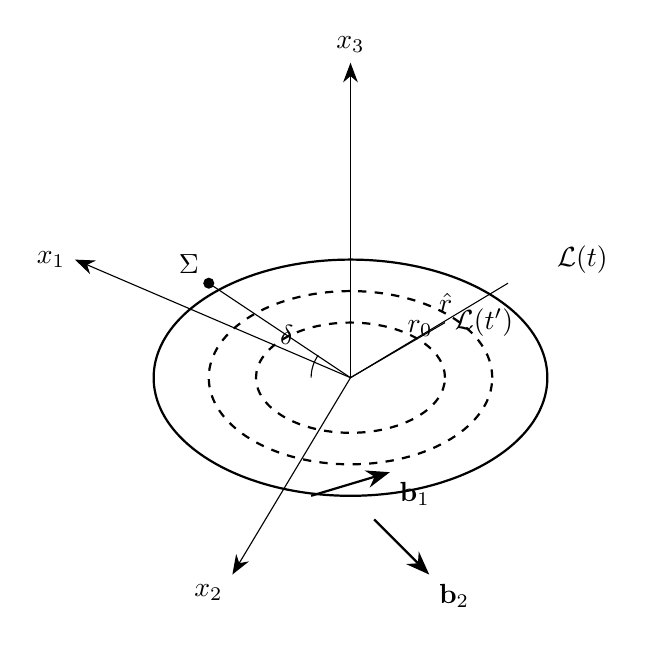
\begin{tikzpicture}[scale=1.0]
    % Оси координат
    \draw[axis] (0,0) -- (0,4);
    \node[above] at (0,4) {$x_3$};
    
    \draw[axis] (0,0) -- (-3.5,1.5);
    \node[left] at (-3.5,1.5) {$x_1$};
    
    \draw[axis] (0,0) -- (-1.5,-2.5);
    \node[below left] at (-1.5,-2.5) {$x_2$};
    
    % Центр окружностей
    \coordinate (O) at (0,0);
    
    % Внутренняя окружность L(t')
    \draw[thick, dashed] (O) ellipse (1.2 and 0.7);
    \node[right] at (1.2, 0.7) {$\mathcal{L}(t')$};
    
    % Средняя окружность
    \draw[thick, dashed] (O) ellipse (1.8 and 1.1);
    
    % Внешняя окружность L(t)
    \draw[thick] (O) ellipse (2.5 and 1.5);
    \node[right] at (2.5, 1.5) {$\mathcal{L}(t)$};
    
    % Радиус r0
    \draw[thin] (O) -- (1.2, 0.7);
    \node[above right] at (0.6, 0.4) {$r_0$};
    
    % Радиус r-hat
    \draw[thin] (O) -- (2.0, 1.2);
    \node[above right] at (1.0, 0.7) {$\hat{r}$};
    
    % Точка Sigma на внешней окружности
    \coordinate (Sigma) at (-1.8, 1.2);
    \fill (Sigma) circle (2pt);
    \node[above left] at (Sigma) {$\Sigma$};
    
    % Угол delta
    \draw[thin] (O) -- (Sigma);
    \draw[thin] (-0.5, 0) arc (180:145:0.5);
    \node[above left] at (-0.6, 0.3) {$\delta$};
    
    % Вектор b1 (винтовая компонента, вдоль касательной)
    \draw[vector] (-0.5, -1.5) -- (0.5, -1.2);
    \node[below right] at (0.5, -1.2) {$\mathbf{b}_1$};
    
    % Вектор b2 (краевая компонента, перпендикулярно)
    \draw[vector] (0.3, -1.8) -- (1.0, -2.5);
    \node[below right] at (1.0, -2.5) {$\mathbf{b}_2$};
\end{tikzpicture}
\caption{Expanding circular loop with coordinate system and Burgers vectors.}
\label{fig:2}
\end{figure}

Referring to (1) and looking at the strain component $U_{2,3}$ we have the non-zero terms:
\begin{multline*}
U_{2,3} = \int_{-\infty}^{t}dt'\int_{L(t')}\left[\frac{b_2}{4\pi}\frac{\partial}{\partial x_1}\left(\frac{1}{\bar{r}}\delta\left(\bar{t}-\frac{\bar{r}}{c_2}\right)\right) + \frac{b_2 c_1^2}{4\pi c_2^2}\frac{\partial}{\partial x_2}\left(\frac{1}{\bar{r}}\delta\left(\bar{t}-\frac{\bar{r}}{c_2}\right)\right)\right]dl_2 \\
+ \int_{-\infty}^{t}dt'\int_{L(t')}\left[\frac{b_2}{4\pi c_2^2}\frac{\partial}{\partial t}\left(\frac{1}{\bar{r}}\delta\left(\bar{t}-\frac{\bar{r}}{c_2}\right)\right)\right](v_1\,dl_2 - v_2\,dl_1).
\end{multline*}

For the field point $P$ we have $\sigma_0=0$, $\zeta=(\cos\delta,0,\sin\delta)$, and by using the length parameter $s=\sigma\hat{r}=\sigma(r_0+\frac{1}{2}at^2)$, instead of the angle $\sigma$, expressions (7) for this case become:
\[
\mathbf{v}=(v,0,0), \quad \mathbf{a}=(a,0,0), \quad \mathbf{p}=(0,1,0), \quad \mathbf{q}=\left(-\frac{1}{\hat{r}},0,0\right), \quad \mathbf{d}=(0,0,0),
\]
where
\[
\hat{r} = r_0 + \tfrac{1}{2}at^2.
\]

However, since in the case of a circular loop the use of the angle $\sigma$ ($0\leqslant\sigma\leqslant 2\pi$) is intuitive we will be evaluating the coefficients of the singular terms by making use of the angle $\sigma$. Accordingly we have
\[
\mathbf{v}=(v,0,0), \quad \mathbf{a}=(a,0,0), \quad \mathbf{p}=(0,\hat{r},0), \quad \mathbf{q}=(-\hat{r},0,0), \quad \mathbf{d}=(0,v,0),
\]
where $\hat{r}=r_0+\frac{1}{2}at^2$ for which (6) yield
\begin{align*}
\mathbf{W} &= (y\cos\delta + \tfrac{1}{2}\hat{r}\theta, -\hat{r}, y\sin\delta), \\
\mathbf{R} &= (\operatorname{sgn}(\theta)y\cos\delta + \tfrac{1}{2}(\hat{r}-a\Lambda^2|\mathbf{W}|)\theta + \Lambda|\mathbf{w}|v, -\hat{r}\operatorname{sgn}(\theta), \operatorname{sgn}(\theta)y\sin\delta), \\
\mathbf{V}^M &= (\mathbf{v}-a\Lambda|\mathbf{W}||\theta|, v\theta, 0),
\end{align*}
\begin{align*}
\mathbf{P} &= (-\hat{r}\theta, \hat{r}-v\Lambda|\mathbf{W}|\theta, 0), \\
\mathbf{A} &= (a, a\theta, 0), \\
\mathbf{D} &= (v\theta, v-a\Lambda|\mathbf{W}||\theta|, 0), \\
\Delta &= (c^2-V^2)\Lambda|\mathbf{W}| - \operatorname{sgn}(\theta)yv\cos\delta + (\tfrac{3}{2}av\Lambda^2|\mathbf{W}|^2 + \tfrac{1}{2}\hat{r}v)|\theta| \\
&\quad + a\cos\delta\Lambda|\mathbf{W}|y\theta + \tfrac{1}{2}\hat{r}a\Lambda|\mathbf{W}|\theta^2,
\end{align*}
so that the inclusion of the coefficients in (3) gives the final result
\begin{equation}
U_{2,3}(P) = \left[\frac{b_2 c_2}{2\pi}\frac{\sqrt{c_2^2-v^2}\cos\delta}{(c_2^2-v^2\sin^2\delta)}\right]\frac{1}{\varepsilon} + \left[\frac{b_2 c_2}{4\pi}\frac{a}{(c_2^2-v^2)^{3/2}} - \frac{b_2}{4\pi c_2}\frac{c_2^2-2c_1^2}{(c_2^2-v^2)^{1/2}\hat{r}}\right]\ln\varepsilon.
\end{equation}

The coefficient of the $1/\varepsilon$ term in (11) coincides with the coefficient of the $1/\varepsilon$ term of a straight screw dislocation tangent to the loop at the point $\Sigma$ and moving with the loop. This in turn coincides with the steady-state solution for this tangent screw dislocation moving with the instantaneous velocity $\mathbf{v}$ as discussed by Clifton and Markenscoff (1981). The coefficient of the $\ln\varepsilon$ term comprises two terms: one involving the acceleration $\mathbf{a}$, which coincides with the coefficient of the $\ln\varepsilon$ term of the tangent straight screw dislocation obtained by Callias and Markenscoff (1988), and one involving the radius of curvature $\hat{r}$ of the loop at time $t$. This last term is new; obviously as $\hat{r}\to\infty$ the loop reduces to a straight screw and this term vanishes as it should. There is no term depending on $\mathbf{d}=\mathrm{d}\mathbf{p}/\mathrm{d}t$, in this example, since $\mathrm{d}\mathbf{p}/\mathrm{d}t$ for a uniformly expanding circular loop is zero.

\subsection*{Case (ii): $b_1 \neq 0$ (Fig. 2)}

In this case the calculation for obtaining the coefficients of the singular terms $1/\varepsilon$ and $\ln\varepsilon$ are cumbersome. Since the coefficient of the $1/\varepsilon$ term should coincide with the one for a straight edge dislocation tangent to the loop at $\Sigma$, as it does for the case $i$ ($b_2\neq 0$), we only checked it for one field point and found it in agreement with the expressions provided for this case by Clifton and Markenscoff (1981). We present here only the calculations for the $\ln\varepsilon$ term which is new.

For instance, looking at the displacement gradient $U_{3,1}$ we have from (1)
\[
U_{3,1} = \int_{-\infty}^{t}dt'\int_{L(t')} C_{1313}b_1(G_{33,1}+G_{13,3})\,dl_2.
\]

For the $\ln\varepsilon$ the non-zero contributions of $G_{33,1}$ are due to $F_2$, $F_3$, $F_4$, $F_5$ and of $G_{13,3}$ are due to $F_2$, $F_5$ and after considerable but straightforward calculation we obtain as the coefficient of the logarithmic term
\begin{multline*}
\left(\frac{b_1 c_2^2}{2\pi v^2}\right)\frac{1}{\hat{r}}\left[\frac{1}{(1-\alpha^2)^{1/2}} - \frac{(1-\frac{3}{2}\beta^2)}{(1-\beta^2)^{3/2}}\right] \\
+ a\left(\frac{3b_1 c_2^2}{2\pi v^4}\right)\left[\frac{(2\beta^2-1)(3\beta^2-4)}{(1-\beta^2)^{1/2}} - \frac{(2\alpha^2-1)(3\alpha^2-4)}{(1-\alpha^2)^{1/2}}\right] \\
+ a\left(\frac{b_1 c_2^2}{\pi v^4}\right)\left[\frac{\alpha^4}{2(1-\alpha^2)^{3/2}} - \frac{\beta^4(\frac{1}{4}-\beta^2)}{(1-\beta^2)^{5/2}}\right],
\end{multline*}
where
\[
\alpha = \frac{v}{c_1} \quad \text{and} \quad \beta = \frac{v}{c_2}.
\]

Again we have here two types of terms either depending on the acceleration $\mathbf{a}$ or the curvature $1/\hat{r}$ and vanishing when either of these quantities vanishes, as discussed in the previous paragraphs.

In conclusion we can say that we have analysed the singular nature of the stress field near an arbitrarily moving dislocation loop and found that it can be approximated by its tangent and its osculating circle at that point. This holds independently of the planarity of the loop.

\section*{Acknowledgement}

One of the authors, Luqun Ni, was supported in part by the Center of Excellence for Advanced Materials at the University of California, San Diego, California, U.S.A.

\section*{References}

\begin{description}
\item[Barnett, D. M.] 1976 \textit{Phys. Statist. Solids} (a) \textbf{38}, 637.
\item[Callias, C. and Markenscoff, X.] 1988 \textit{Archs ration. Mech. Anal.} \textbf{102}, 273.
\item[Callias, C., Markenscoff, X. and Ni, L.] 1989 The Singularity of the Near-field of an Arbitrarily Moving Dislocation Loop, \textit{Q. appl. Math.}, in press.
\item[Clifton, R. J. and Markenscoff, X.] 1981 \textit{J. Mech. Phys. Solids} \textbf{29}, 227.
\item[G\"unther, H.] 1968 \textit{Annalen der Physik} \textbf{21}, 93.
\item[Madariaga, R.] 1976 \textit{Bull. Seism. Soc. Am.} \textbf{66}, 639.
\item[Markenscoff, X. and Clifton, R. J.] 1982 \textit{J. appl. Mech.} \textbf{49}, 792.
\item[Markenscoff, X. and Ni, L.] 1984a \textit{Q. appl. math.} \textbf{41}, 475.
\item[Markenscoff, X. and Ni, L.] 1984b \textit{J. appl. Mech.} \textbf{51}, 753.
\item[Mura, T.] 1963 \textit{Phil. Mag.} \textbf{8}, 843.
\item[Mura, T.] 1969 In \textit{Mathematical Theory of Dislocations} (edited by T. Mura), pp. 25--48, ASME.
\end{description}

\section*{Appendix}

\begin{multline}
F_1(\theta,y,C_i) = \left(\frac{\varepsilon_{njh}C_{ijkl}b_i}{4\pi\rho}\right)\frac{R_k R_m R_l}{C_i^3\Lambda^2|\mathbf{W}|^2\Delta^3}(P_h(\mathbf{R},\mathbf{A}) + D_h\Delta_2) \\
- \left(\frac{b_i\varepsilon_{nrs}}{4\pi}\right)\left[\frac{R_i R_m}{C_i\Lambda|\mathbf{W}|\Delta^2}(A_r P_s + V_r^M D_s) + \frac{R_i R_m}{C_i\Lambda|\mathbf{W}|\Delta^3}\right](\mathbf{R},\mathbf{A})V_r^M P_s,
\end{multline}

\begin{multline}
F_2(\theta,y,C_i) = \left(\frac{-\varepsilon_{njh}C_{ijkl}b_i}{4\pi\rho}\right)\frac{P_h}{C_i^3\Lambda^2|\mathbf{W}|^2\Delta} \\
\times \left[\frac{1}{\Delta}(R_l R_m V_k^M + R_l R_k V_m^M + R_k R_m V_l^M) + (\delta_{km}R_l + \delta_{ml}R_k + \delta_{kl}R_m) \right. \\
\left. + R_l R_m R_k\left(\frac{2}{\Lambda|\mathbf{W}|\Delta} - \frac{1}{\Delta^2}(C_i^2 - (\mathbf{V}^M,\mathbf{V}^M)) - \frac{3}{C_i^2\Lambda^2|\mathbf{W}|^2}\right)\right] \\
+ \left(\frac{b_i\varepsilon_{nrs}}{4\pi}\right)P_s V_r^M\left[\frac{V_i^M R_m + R_i V_m^M}{C_i\Lambda|\mathbf{W}|\Delta^2}
 - \frac{3R_i R_m}{C_i\Lambda^2|\mathbf{W}|^2\Delta^2}\right. \\
\left.
     + \frac{\delta_{im}}{C_i\Lambda|\mathbf{W}|\Delta}
 - \frac{R_i R_m(\mathbf{R},\mathbf{V}^M)^2}{C_i^3\Lambda^3|\mathbf{W}|^3\Delta^3}
 + \frac{R_i R_m(\mathbf{V}^M,\mathbf{V}^M)}{C_1\Lambda|\mathbf{W}|\Delta^3}\right],
\end{multline}

\begin{multline}
F_3(\theta,y,c_2) = -\left(\frac{\varepsilon_{njh}C_{ijkl}b_i}{4\pi\rho c_2}\right)\left[\frac{R_l D_h}{\Delta^2} + \frac{P_h R_l(\mathbf{R},\mathbf{A})}{\Delta^3}\right]\delta_{km} \\
+ \left(\frac{b_i\varepsilon_{nrs}}{4\pi}\right)\frac{c_2\Lambda\mathbf{W}}{\Delta^3}\left[(D_s V_r^M + P_s A_r)\Delta + P_s V_r(\mathbf{R},\mathbf{A})\right]\delta_{lm},
\end{multline}

\begin{multline}
F_4(\theta,y,c_2) = \left(\frac{\varepsilon_{njh}C_{ijkl}b_i}{4\pi\rho c_2}\right)\left[\frac{P_h V_l^M}{\Delta^2} - \frac{R_l P_h}{\Delta^3}(c_2^2 - (\mathbf{V}^M,\mathbf{V}^M))\right]\delta_{km} \\
+ \left(\frac{b_i\varepsilon_{nrs}c_2}{4\pi}\right)\left[\frac{(\mathbf{R},\mathbf{V}^M) - c_2^2\Lambda\mathbf{W}(\mathbf{V},\mathbf{V})}{\Delta^3}\right]P_s V_r^M\delta_{lm},
\end{multline}

\begin{multline}
F_5(\theta,y,c) = \int_0^{\Lambda}|\mathbf{W}|\,du\left\{\left(\frac{\varepsilon_{njh}C_{ijkl}b_i}{4\pi\rho}\right)P_h'|\mathbf{W}|u \right. \\
\left. \times \left[\frac{3(\delta_{mk}R_l' + \delta_{kl}R_n' + \delta_{ml}R_k')}{R'^5} - \frac{15R_l'R_m'R_k'}{R'^7}\right] + \left(\frac{b_i\varepsilon_{nrs}}{4\pi}\right)V_r'P_s'\left(\frac{3R_l'R_m'}{R'^5} - \frac{\delta_{lm}}{R'^3}\right)\right\},
\end{multline}
with
\begin{align*}
\mathbf{P}' &= \mathbf{p} + \mathbf{q}\theta - \mathbf{d}|\theta||\mathbf{W}|u, \\
\mathbf{V}' &= \mathbf{v} + \mathbf{d}\theta - \mathbf{a}|\theta||\mathbf{W}|u, \\
\mathbf{R}' &= \frac{\theta}{|\theta|}\mathbf{W} + (\mathbf{v}+\mathbf{d}\theta - \tfrac{1}{2}\mathbf{a}|\theta||\mathbf{W}|u)|\mathbf{W}|u, \\
R' &= (\mathbf{R}',\mathbf{R}')^{1/2}.
\end{align*}

\end{document}
